\begin{figure}
\centering
\begin{subfigure}{.23\textwidth}
  \centering
  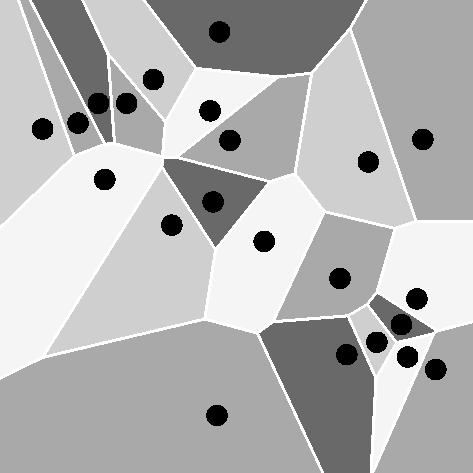
\includegraphics[width=\linewidth]{voronoi0.pdf}
  \caption{$\text{dgm}_{\Vor}(X)$.}
\end{subfigure}
\hfill
\begin{subfigure}{.23\textwidth}
  \centering
  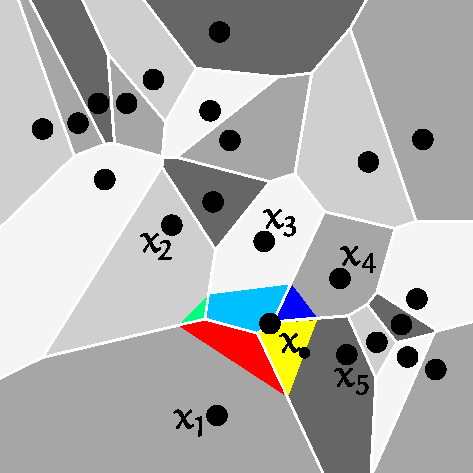
\includegraphics[width=\linewidth]{voronoi1.pdf}
  \caption{Inserting a point.}
\end{subfigure}
\hfill
\begin{subfigure}{.23\textwidth}
  \vspace{0.2cm}
  \centering
  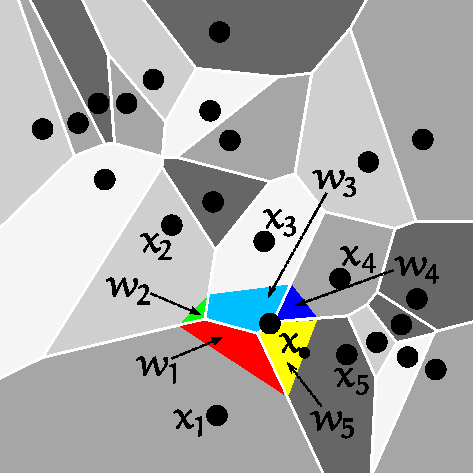
\includegraphics[width=\linewidth]{voronoi2.pdf}
  \caption{Cells $\Vor(x_i)$.}
\end{subfigure}
\hfill
\begin{subfigure}{.23\textwidth}
  \vspace{0.2cm}
  \centering
  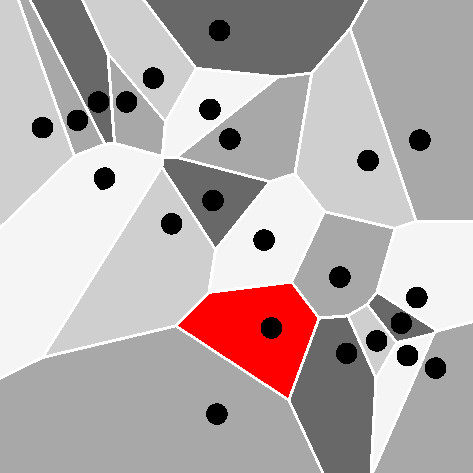
\includegraphics[width=\linewidth]{voronoi3.pdf}
  \caption{$\text{dgm}_{\Vor}(X \cup x_\bullet)$.}
\end{subfigure}
\caption{(a) Clipped version of the Voronoi tesselation. For arbitrary manifolds the curvature must be considered for a correct clip. (b) Tesselation with an added point, which creates a new Voronoi region, \textit{stealing} parts of the neighboring regions $x_1, \ldots, x_5 \in \mathbb{R}^d$. (c) The determined weights $w_1, \ldots, w_5 \in \mathbb{R_+}$ by the fractional amount of occupied volume. (d) Tesselation with an added point.}
\label{fig:voronoi}
\end{figure}